\section{Overview}\label{sec:overview}

\begin{figure}
  \centering
  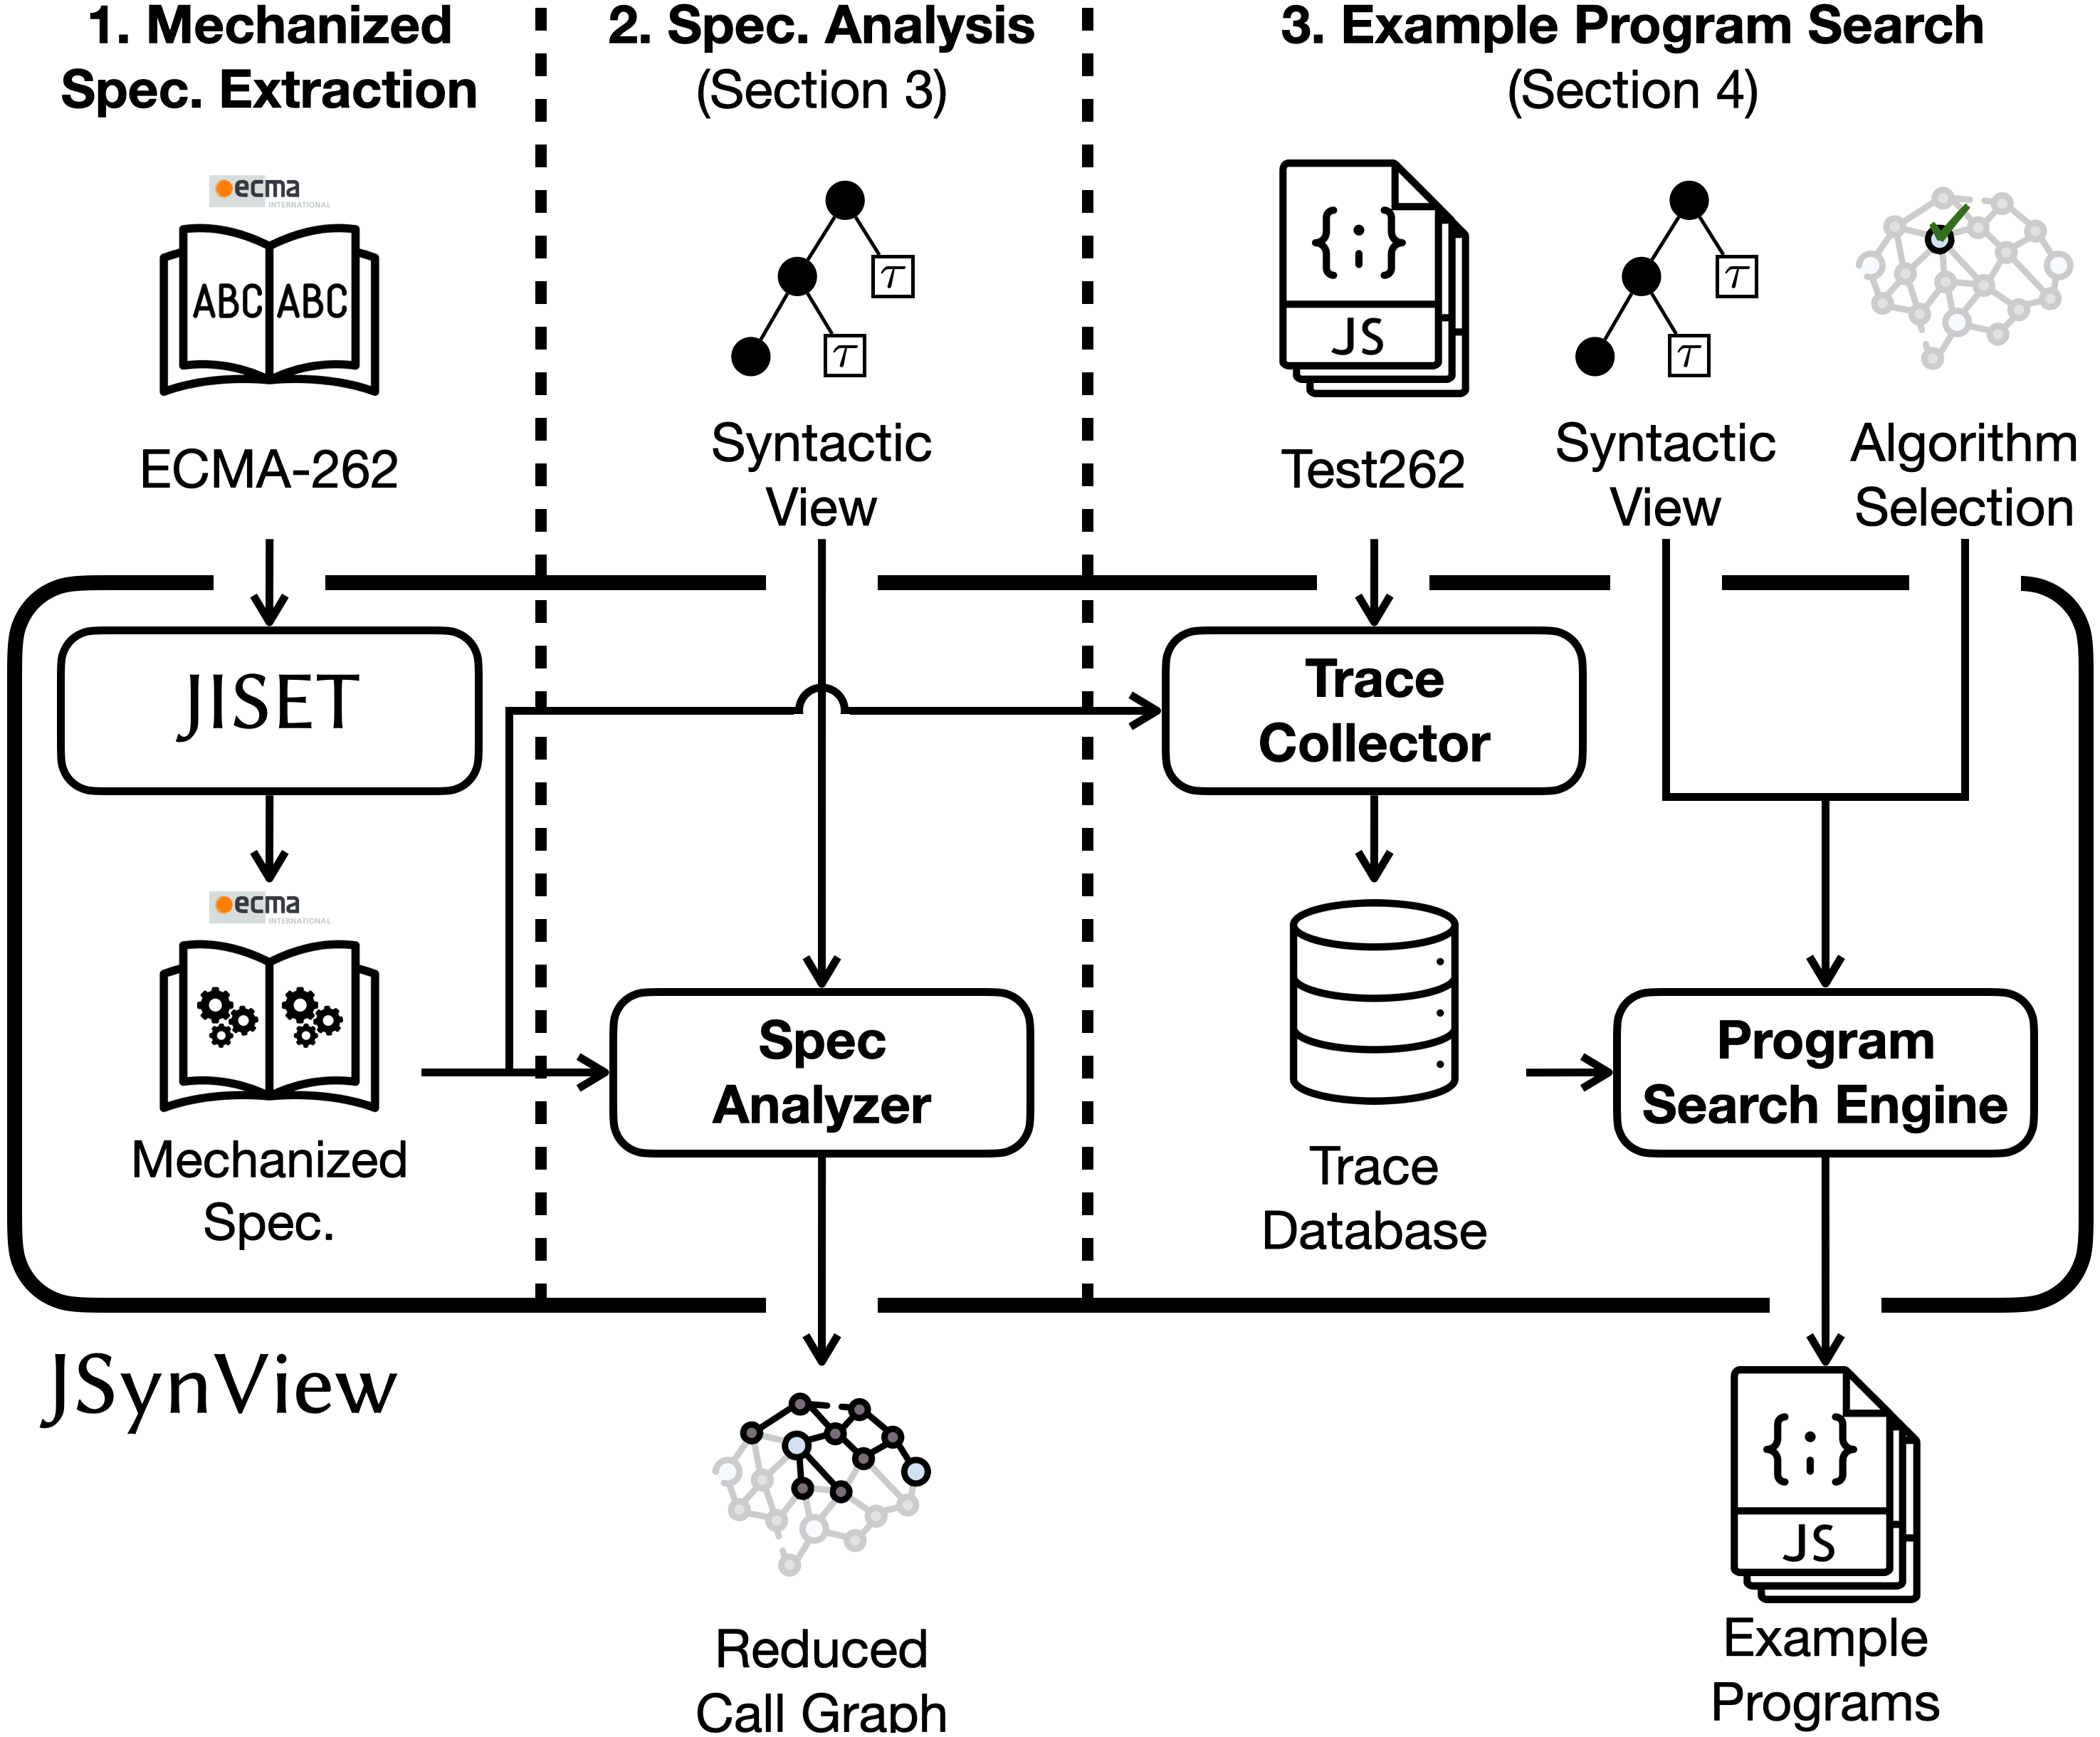
\includegraphics[width=\columnwidth]{img/overall.png}
  \caption{Overall structure of $\tool$}
  \vspace*{-1em}
  \label{fig:overall}.
\end{figure}

This section explains the overall structure of $\tool$ depicted in
Figure~\ref{fig:overall} with simple examples.  It consists of three phases: 1)
\textit{mechanized specification extraction}, 2) \textit{behavior inference} and
3) \textit{example program search}.

\subsection{Mechanized Specification Extraction}\label{sec:extract-spec}

\begin{figure}
  \centering
  \begin{subfigure}[t]{\columnwidth}
    \centering
    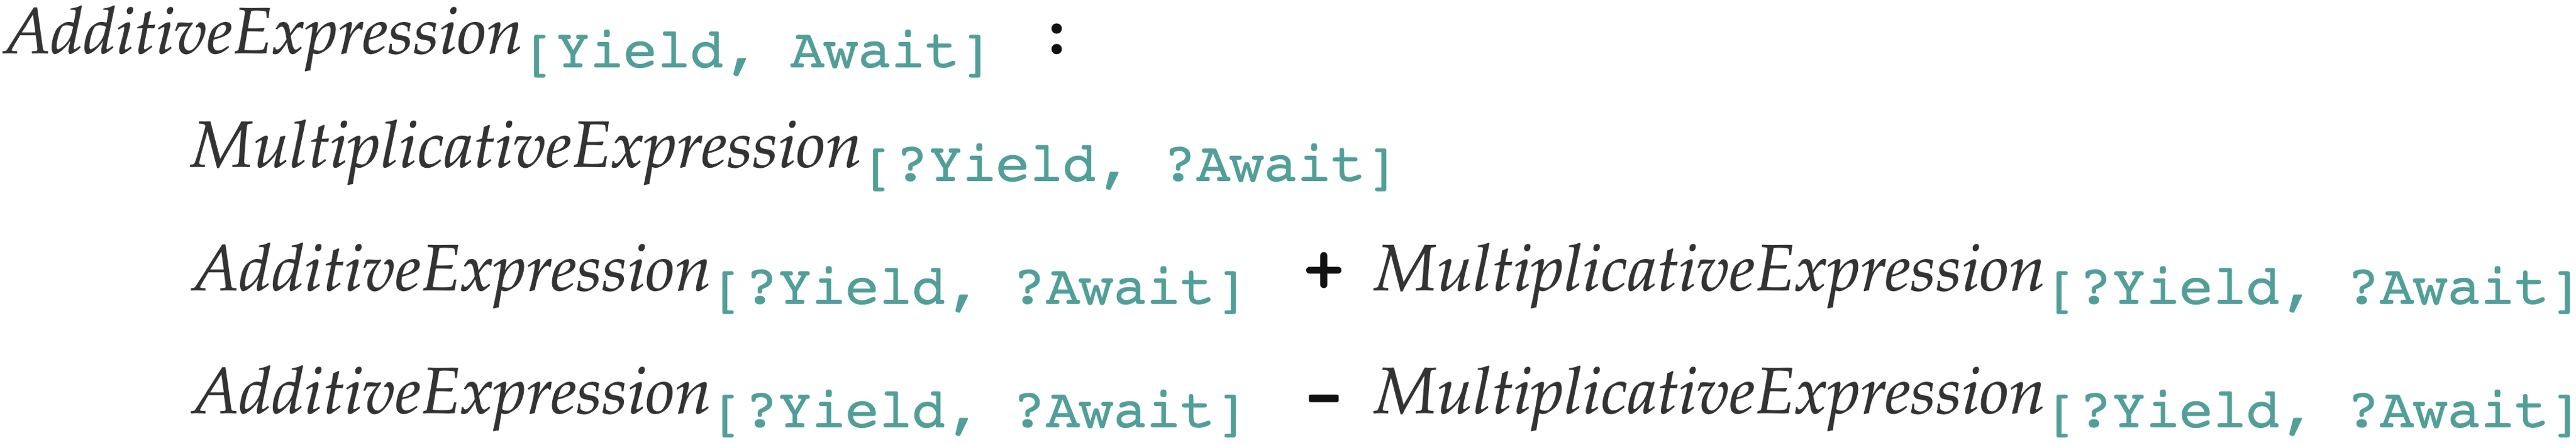
\includegraphics[width=\columnwidth]{img/add-eval-bnf.png}
    \caption{The \essyn{AdditiveExpression} production for syntax}
    \label{fig:add-eval-bnf}
  \end{subfigure}
  \begin{subfigure}[t]{\columnwidth}
    \centering
    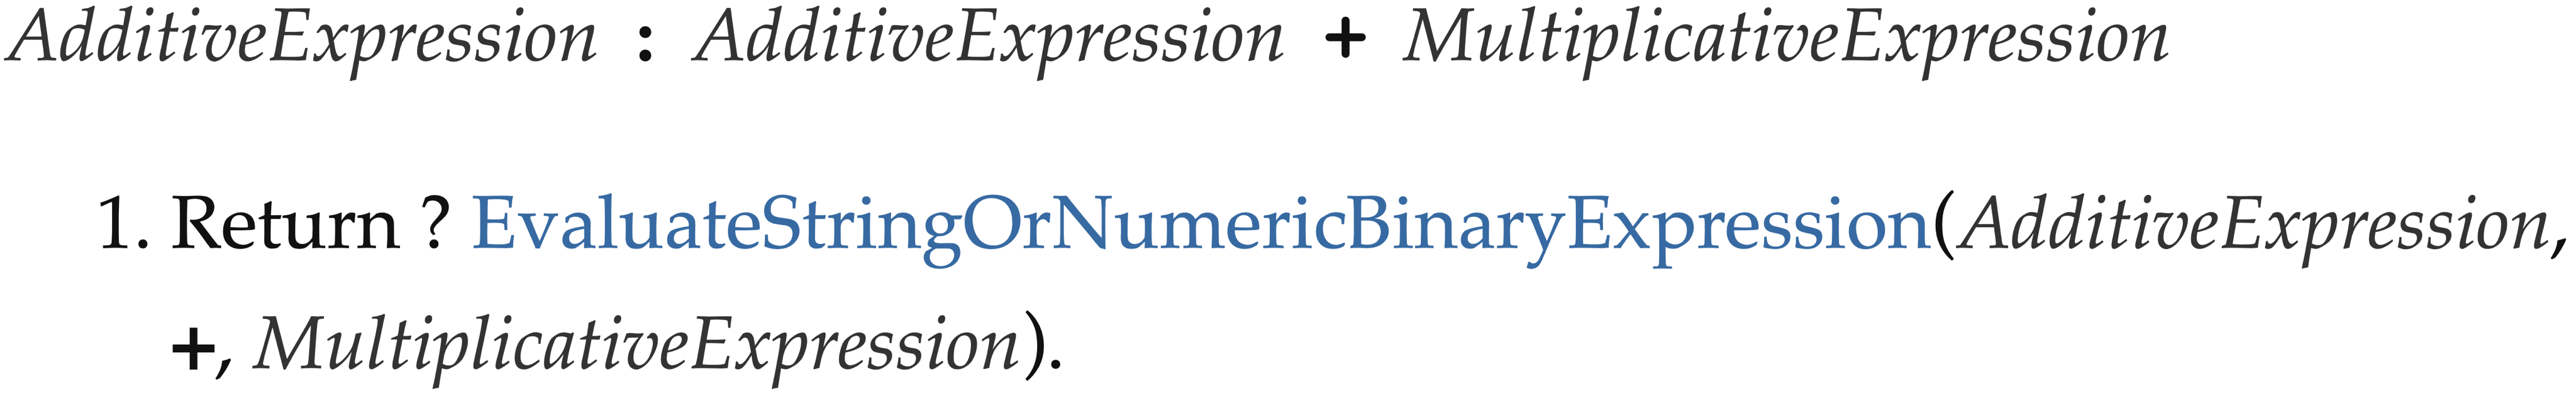
\includegraphics[width=\columnwidth]{img/add-eval-algo.png}
    \caption{The \esalg{Evaluation} algorithm of for semantics}
    \label{fig:add-eval-algo}
  \end{subfigure}
  \caption{The syntax and semantics of the addition expression in the latest
  ECMA-262 (ES12, 2021)}
  \vspace*{-1em}
  \label{fig:add-eval}
\end{figure}

$\tool$ first extracts a \textit{mechanized specification} from ECMA-262, the
standard JavaScript language specification written in English.

ECMA-262 describes the syntax using a variant of the extended Backus–Naur form
and the semantics as abstract algorithms.  Each algorithm describes the language
semantic in a procedural way with structured steps.  For example,
Figure~\ref{fig:add-eval-bnf} shows the syntactic production of
\essyn{AdditiveExpression} in the latest ECMA-262 (ES12, 2021)~\cite{es12}.
Figure~\ref{fig:add-eval-algo} shows the \esalg{Evaluation} algorithm of its
second alternative that describes the semantics of the addition
expression.\footnote{\url{https://262.ecma-international.org/12.0/\#sec-addition-operator-plus}}
It consists of a single step that invokes another algorithm,
\esalg{EvaluateStringOrNumericBinaryExpression}; the first and third arguments
are the left and right subtrees of the abstract syntax tree (AST) for a given
addition expression, and the second one is a text \code{+} to represent the
addition operation.  The \esalg{EvaluateStringOrNumericBinaryExpression} is a
generic algorithm for string or numeric binary operations (e.g., \code{-},
\code{*}, \code{<}, etc.).

However, it is difficult to handle it in an automatic or mechanical way since it
is written in English.  Thus, we utilize another tool $\jiset$~\cite{jiset},
which extracts a mechanized specification from any given version of ECMA-262.
It automatically converts algorithms steps to the corresponding instructions of
$\ires$, an intermediate representation for ECMAScript.  In other word, the
mechanized specification extracted via $\jiset$ is an $\ires$ program consisting
of functions corresponding to abstract algorithms in the language specification.
In this paper, we use its newer platform $\esmeta$~\cite{esmeta}, an
\underline{E}CMAScript \underline{S}pecification \underline{M}etalanguage,
because it is more actively maintained rather than $\jiset$.


\subsection{Behavior Inference}\label{sec:reduce-spec}

\begin{figure}
  \centering
  \begin{subfigure}[t]{\columnwidth}
    \centering
    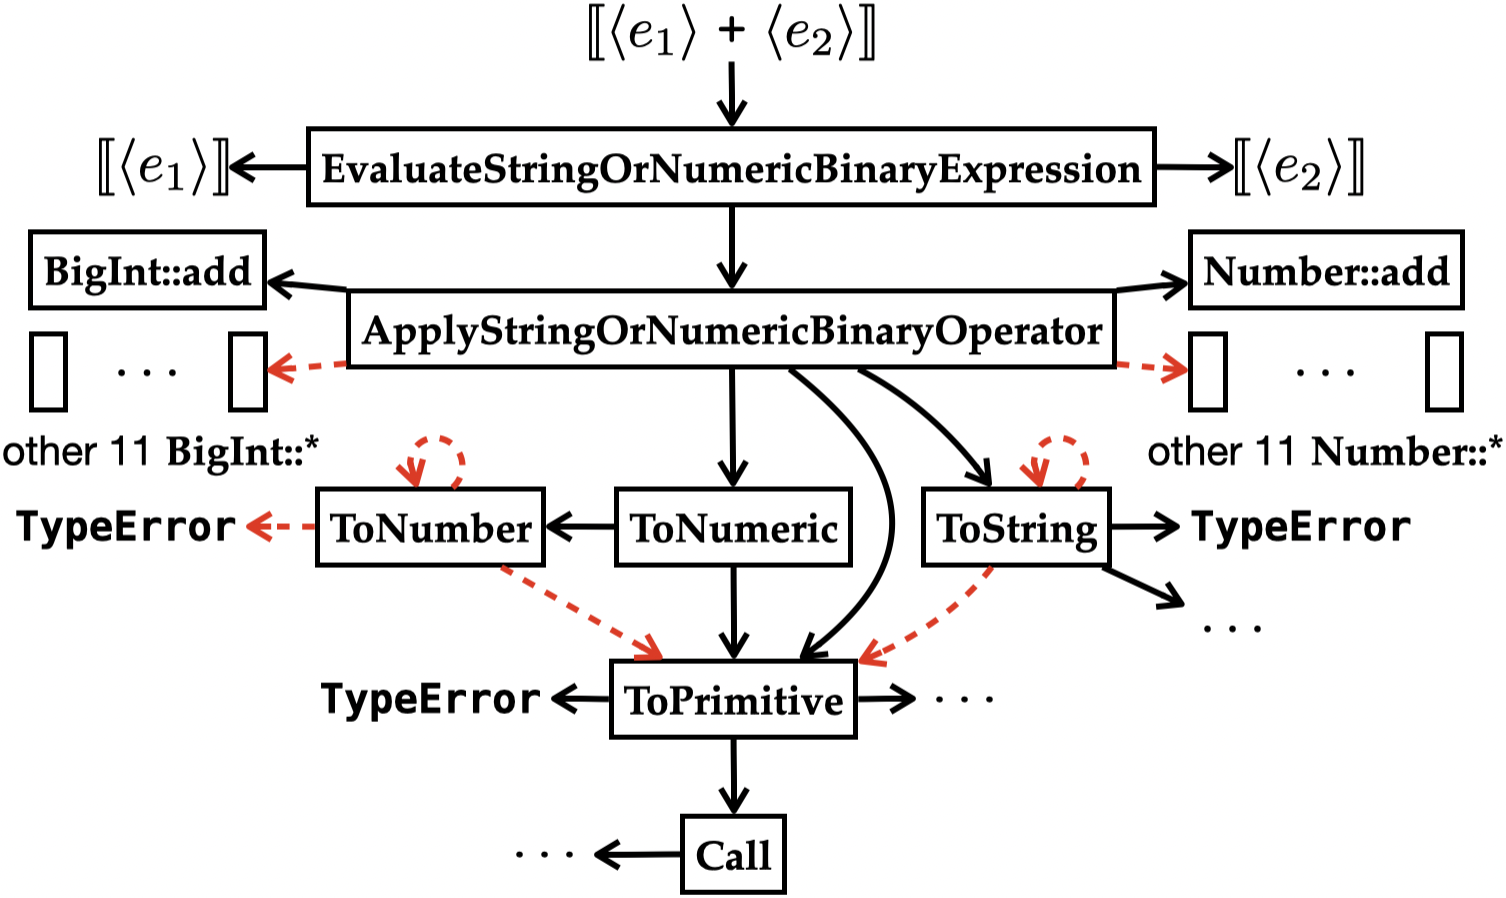
\includegraphics[width=\textwidth]{img/add-basic.png}
    \caption{Reduced call graph with $\svhole{\expr_1} \; \code{+} \;
    \svhole{\expr_2}$}
    \label{fig:add-basic-graph}.
  \end{subfigure}
  \begin{subfigure}[t]{\columnwidth}
    \centering
    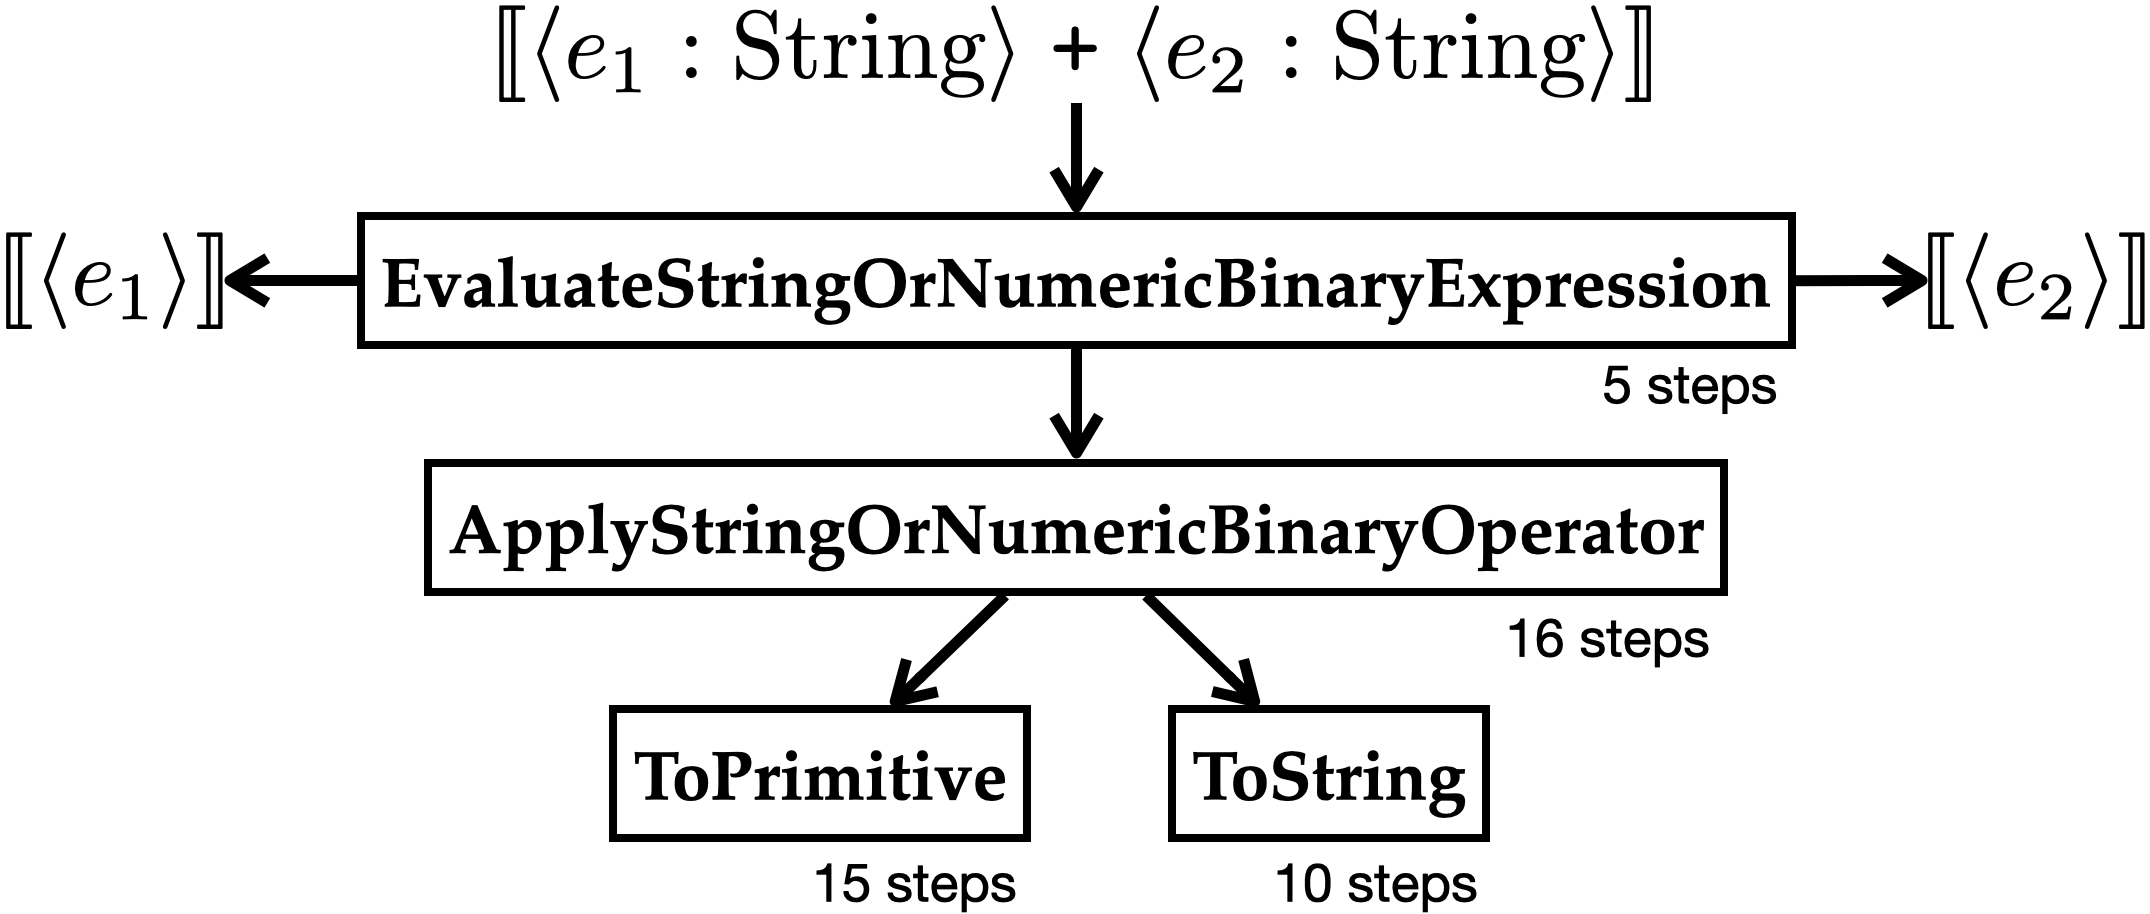
\includegraphics[width=.8\textwidth]{img/add-str.png}
    \caption{Reduced call graph with $\svhole{\expr_1: \text{String}} \;
    \code{+} \; \svhole{\expr_2: \text{String}}$}
    \label{fig:add-str-graph}.
  \end{subfigure}
  \caption{A call graph of the JavaScript language specification reduced with
    two different syntactic views}
  \vspace*{-1em}
  \label{fig:add-graph}.
\end{figure}

After extracting the mechanized specification, the \textit{Reachability
Analyzer} performs static analysis for the mechanized specification extracted
from ECMA-262.  Then, it automatically infers \textit{possible behaviors} of
language features using the analysis results.  Users can select the target
language feature they want to understand by defining a \textit{syntactic view},
which is an extension of a JavaScript AST with abstract nodes and optional type
bounds.  It restricts syntax and expected types of evaluation results of
JavaScript programs.  For example, assume that we want to understand the
detailed semantics of JavaScript addition operator (\code{+}) by referring to
the latest ECMA-262 (ES12, 2021).  To repesent this language feature, we can
utilize a syntactic view $\svhole{\expr_1} \; \code{+} \; \svhole{\expr_2}$
where $\svhole{\expr_1}$ and $\svhole{\expr_2}$ denote arbitrary expressions
without any type bounds.  For this syntactic view, the reachability analyzer
first finds \esalg{Evaluation} algorithm of the addition operator shown in
Figure~\ref{fig:add-eval-algo} as the initial point of the analysis.  Then, it
builds reduced call graphs consisting of the algorithms only reachable from the
initial algorithm.

Figure~\ref{fig:add-basic-graph} depicts the a call graph built by following all
algorithms starting from the \esalg{Evaluation} algorithm.  In this graph, a
node denotes 1) an abstract algorithm (box), 2) evaluation of syntactic view
($\sem{-}$), or 3) an exception (bold without box), and an arrow denotes a call
edge.  Among them, specific algorithms represent possible behaviors of the
addition operator.  For instance, the \esalg{Call} algorithm is used to call the
\eswrd{[[Call]]} internal method of a JavaScript function object.  It means that
a JavaScript function might be invoked during the evaluation of the addition
operator.  Besides, the addition operator might throw a \esval{TypeError}
exception because it is reachable from the \esalg{Evaluation} algorithm through
\esalg{ToNumber}, \esalg{ToString}, and \esalg{ToPrimitive}.

However, this call graph contains invalid edges for the evaluation of the
addition operator, and red dotted arrows in Figure~\ref{fig:add-basic-graph}
denote such cases.  For example, \esalg{ApplyStringOrNumericBinaryOperator} only
invokes two different numeric methods \esalg{BigInt::add} and
\esalg{Number::add} for the evaluation of the addition operator.  Other 22
numeric methods, such as \esalg{BigInt::subtract} and \esalg{Number::divide},
are unreachable.  Moreover, \esval{TypeError} is throwable only in
\esalg{ToPrimitive} and \esalg{ToString} but not in \esalg{ToNumber} for the
addition operator.

Beyond basic syntactic restriction, we can give a more restriction to a
syntactic view with 1) type bounds or 2) combination with other language
features.  For instance, assume that we want to understand the addition between
string values.  Then, the syntactic view $\svhole{\expr_1: \text{String}} \;
\code{+} \; \svhole{\expr_2: \text{String}}$ represents such cases, and
Figure~\ref{fig:add-str-graph} depicts the reduced call graph with this syntactic
view, and gives more information of the addition operator.  First, the addition
between string values never throws exceptions because there is no reachable
exceptions in this call graph.  Second, the string addition never invoke other
JavaScript functions because the \esalg{Call} algorithm is no longer reachable
from the \esalg{Evaluation} algorithm.  We can even restrict the expected
results of the abstract nodes using exceptions as type bounds: $\svhole{\expr_1:
\bot} \; \code{+} \; \svhole{\expr_2: \bot}$, where $\bot$ denotes an exception:
\begin{figure}[H]
  \centering
  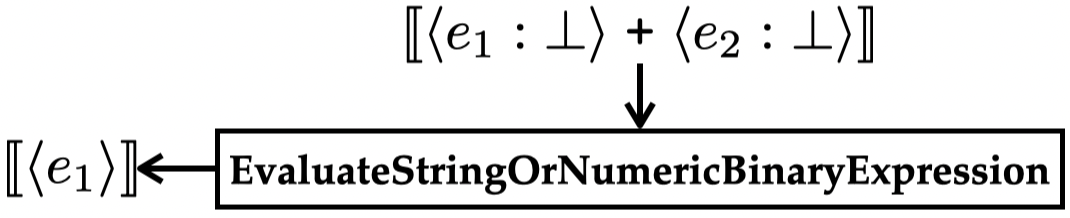
\includegraphics[width=.7\columnwidth]{img/add-exc.png}
\end{figure} \noindent
In this case, we notice that only left operand is evaluated when both left and
right operand throw exceptions.  Besides, we can combine different language
features in syntactic views.  For example, a syntactic view $\svhole{\expr_1:
\text{Number}} \; \code{+} \; \svhole{\expr_2: \text{Number}} \; \code{*} \;
\svhole{\expr_3: \text{Number}}$ represents the combination of numeric addition
and multiplication.





\subsection{Example Program Search}\label{sec:reduce-spec}

Beyond possible behaviors of language features, $\tool$ also provides
\textit{example programs} by searching them in Test262, an official JavaScript
conformance test suite.

The \textit{Trace Collector} first executes all JavaScript programs in Test262
using the mechanized specification extracted from ECMA-262.  Then, it utilizes
their execution traces to build \textit{Trace Database} for reachability
relations between their AST nodes and abstract algorithms of the specification.
For example, consider that a simple addition expression: \jscode{1 + 2}.  After
evaluation of 
The \textit{Program Search Engine} utilizes it to search example programs for a
given syntactic view and a selected algorithm.


Note that the database is built only once before 

collects their
execution traces and 

to .  The database contains the relation
between AST nodes of programs and abstract algorithms in ECMA-262.  Note that 

While the reachability analysis with a given syntactic view provides possible
behaviors of the corresponding language feature, it is another challenging
problem to find concrete example programs that trigger a specific behavior.  For
example,


\begin{itemize}
  \item In Figure~\ref{fig:add-basic-graph}
    \begin{itemize}
      \item TypeError in ToString:
        \code{test/language/expressions/addition/symbol-to-string.js}
      \item Call:
        \code{test/language/expressions/addition/S11.6.1\_A2.2\_T1.js}
    \end{itemize}
\end{itemize}
